\subsection{a}
Rearranging the equation and finding its characteristic equation:
\begin{equation} \label{eq:h(t)}
\begin{split}
    &M \frac{d^2h}{dt^2} + c \frac{dh}{dt} + kh = 0 \implies
        \frac{d^2h}{dt^2} + \frac{c}{M} \frac{dh}{dt} + \frac{k}{M}h = 0 \\
    &\frac{d^2h}{dt^2} + 6 \frac{dh}{dt} + 25 h = 0 \\
    & m^2 + 6m + 25 = 0 \implies m = -3 \pm 4i \\
    \therefore \ & h(t) = e^{-3t} \left( Ae^{4it} + Be^{-4it} \right)
\end{split}
\end{equation}
We are given two initial conditions: $h(0) = 0.15$ and $h'(0) = -0.05$. Using matlab to solve it:
\begin{equation*}
\begin{split}
    &h(t) = {e}^{-3t} \frac{\,{\left(3\,\mathrm{cos}\left(4\,t\right)+2\,\mathrm{sin}\left(4\,t\right)\right)}}{20}
\end{split}
\end{equation*}

\lstinputlisting[caption={Topic 6. Question a}]{"./files/topic6/a.m"}

\pagebreak
As can be seen in Figure \ref{fig:Topic6-b}, between $t = 0$ and approximately $t=0.6$, the suspension is being compressed.
Ultimately it reaches -0.02m, which means that vehicle body is under its normal resting position (conceptually similar to it being above the resting position in the beginning of the movement)
The oscillation is heavily dampened, which means the car does not move up-and-down continuously following the first bump.
This is shown in the graph between about $t=0.7$ and about $t=1.5$.
\subsection{b}
\begin{figure}[h]
	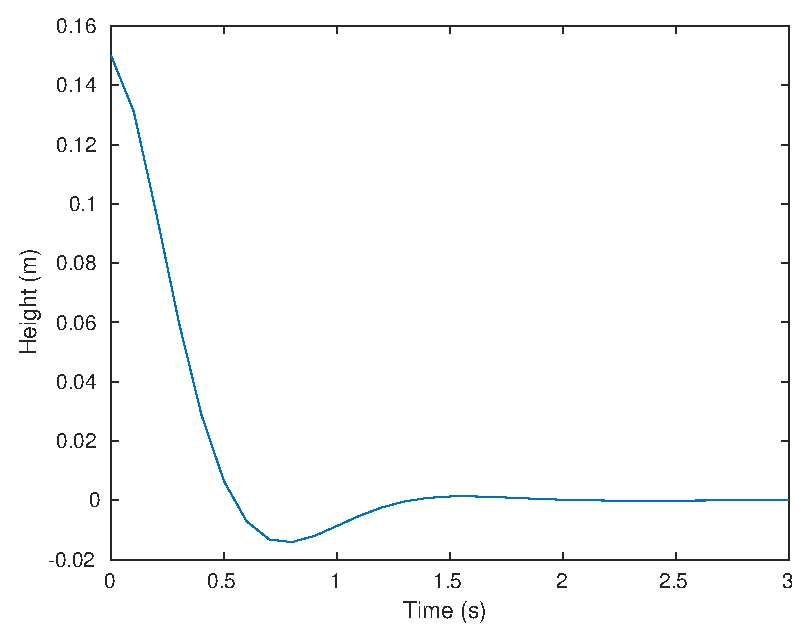
\includegraphics[scale=0.65, center]{./eps/topic6_b.eps}
	\caption{Suspension height during impact}
	\label{fig:Topic6-b}
\end{figure}

\lstinputlisting[caption={Topic 6. Question b. Note this is a continuation of the code for a)}]{"./files/topic6/b.m"}

\subsection{c}
\begin{equation} \label{eq:forcedVibration}
\begin{split}
    \frac{d^2h}{dt^2} + \frac{c}{M} \frac{dh}{dt} + \frac{k}{M}h = \frac{F}{M} e^{i\omega t} \\
    \frac{d^2h}{dt^2} + 6 \frac{dh}{dt} + 25 h = 2.5 e^{i\omega t} \\
\end{split}
\end{equation}

Equation (\ref{eq:h(t)}) gave us the complimentary function. We could find the particular integral manually, however matlab is utilised
\lstinputlisting[caption={Topic 6. Question c (i)}]{"./files/topic6/ci.m"}

General solution
\begin{equation}
    \begin{array}{l}
        C_1 \,\mathrm{cos}\left(4\,t\right)\,{\mathrm{e}}^{-3\,t} -C_2 \,\mathrm{sin}\left(4\,t\right)\,{\mathrm{e}}^{-3\,t} +\frac{5\,{\mathrm{cos}\left(4\,t\right)}^2 \,{\mathrm{e}}^{t\,\omega\,\mathrm{i}} }{\sigma_1 }+\frac{5\,{\mathrm{sin}\left(4\,t\right)}^2 \,{\mathrm{e}}^{t\,\omega\,\mathrm{i}} }{\sigma_1 }\\
        \textrm{where}\\
        \;\;\sigma_1 =2\,{\left(-\omega^2 +6\,\omega\,\mathrm{i}+25\right)}
        \end{array}
\end{equation}

Particular solution
\begin{equation}
    \frac{{\mathrm{e}}^{-3\,t} \,{\left(50\,\mathrm{cos}\left(4\,t\right)+25\,\mathrm{sin}\left(4\,t\right)+100\,{\mathrm{e}}^{t\,{\left(3+\omega\,\mathrm{i}\right)}} -6\,\omega^2 \,\mathrm{cos}\left(4\,t\right)-4\,\omega^2 \,\mathrm{sin}\left(4\,t\right)+36\,\omega\,\mathrm{cos}\left(4\,t\right)\,\mathrm{i}-\omega\,\mathrm{sin}\left(4\,t\right)\,\mathrm{i}\right)}}{40\,{\left(-\omega^2 +6\,\omega\,\mathrm{i}+25\right)}}
\end{equation}

\lstinputlisting[caption={Topic 6. Question c (ii). Note it is the continuation of the code for c (i)}]{"./files/topic6/cii.m"}
\begin{figure}[h]
	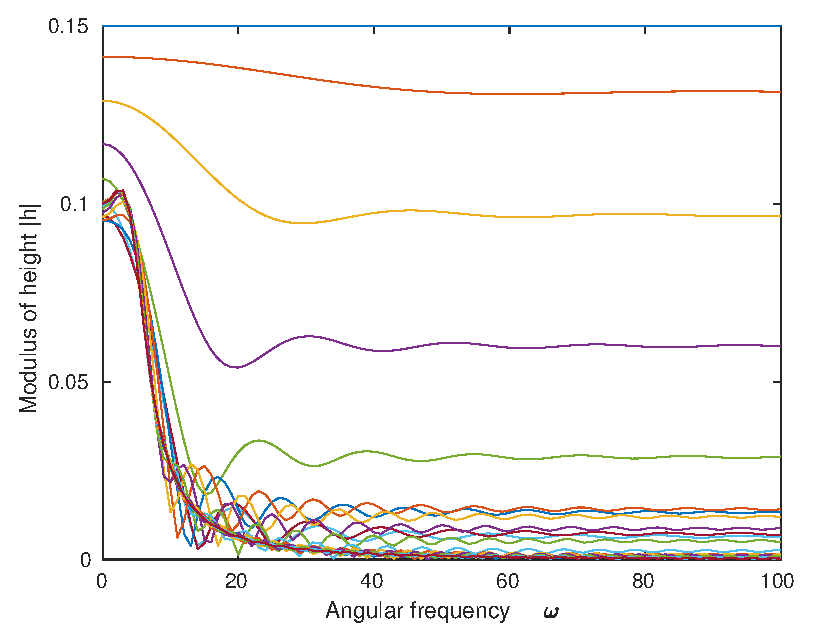
\includegraphics[scale=0.65, center]{./eps/topic6_c.eps}
	\caption{Note that each line represents a distinct moment in time from t=0 to t=2}
	\label{fig:Topic6-b}
\end{figure}

For $\omega$ around 10 to 20, there is heavy oscillation which gets reduced with an increase in the angular frequency.
This suggests that a very large number of bumps on the road "dillutes" the impact -- presumably imitating the conditions of a poorly maintained road.
If the objective is to punish those who choose to go over the grid at higher speeds, then the graph suggests that the grid will achieve that.
Ultimately, there are alternative speed control systems, such as the use of cameras and fines, though their compared effectiveness is up for contention.

\pagebreak